% ===========================================================================
\section{Results}
\label{sec:results}
% ===========================================================================

\subsection{Segment completion matters more than factor revision}

The legacy 2006 calculation is \SI{3.805}{\mega\tonne} \COe{} for FY2019--20 and
\SI{3.317}{\mega\tonne} on FY2023--24 production. Applying 2019 factors to the same FY2023--24
production raises the estimate to \SI{4.485}{\mega\tonne}. Adding gathering and processing
gives \SI{10.095}{\mega\tonne}; the full public-data ledger gives
\SI{23.499}{\mega\tonne}---high in the sector's \SIrange{9.601}{24.694}{\mega\tonne}
structural envelope, whose top keeps fertilizer feedstock inside the post-meter leak base
(Figure~\ref{fig:ladder}). The factor-framework
revision is therefore
smaller than the effect of representing additional supply-chain segments.

\begin{figure}[htbp]
\centering
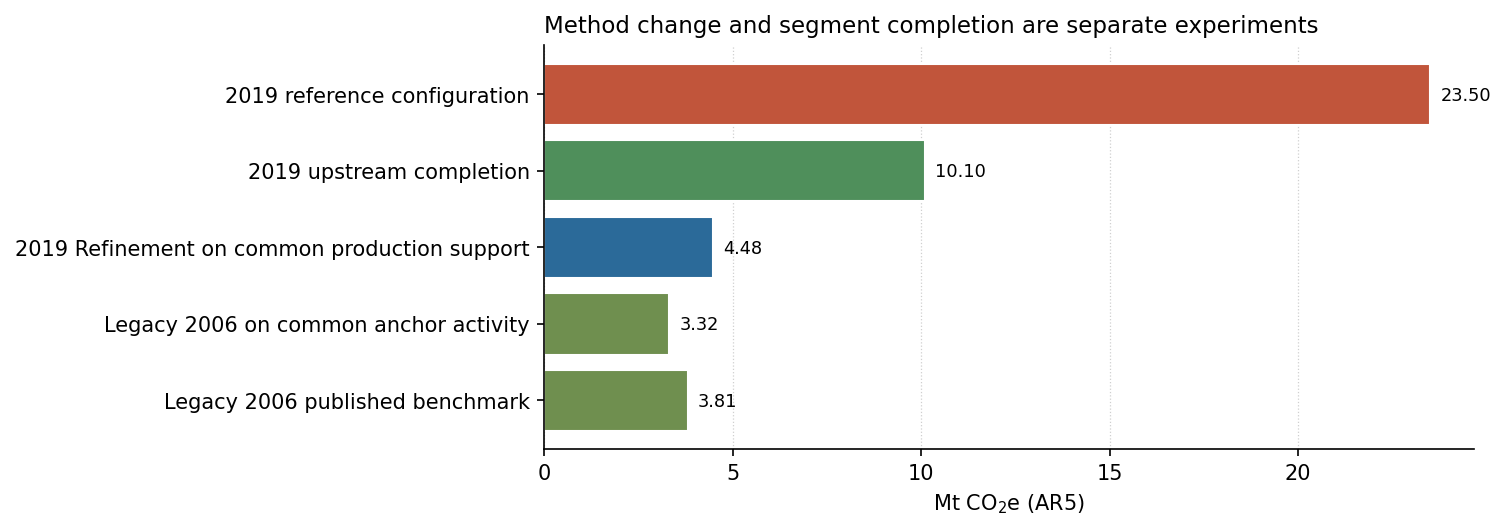
\includegraphics[width=\linewidth]{fugitives_method_ladder.png}
\caption{Method-resolution ladder. Common production support isolates the factor-framework
effect before the account expands to additional segments.}
\label{fig:ladder}
\end{figure}

\subsection{Distribution and post-meter assumptions determine the range}

The reference inventory contains \SI{752.761}{\giga\gram} CH$_4$,
\SI{915.619}{\giga\gram} CO$_2$ and \SI{3.483}{\tonne} N$_2$O
(Table~\ref{tab:segments}). Distribution is the largest segment
(\SI{7.069}{\mega\tonne}), followed by gas production (\SI{4.011}{\mega\tonne}),
post-meter industrial and power use (\SI{3.420}{\mega\tonne}) and gathering
(\SI{3.113}{\mega\tonne}).

\begin{table*}[htbp]
\centering
\scriptsize
\begin{tabular}{@{}lrrrrrl@{}}
\toprule
\textbf{Segment} & \textbf{CH$_4$ (Gg)} & \textbf{CO$_2$ (Gg)} & \textbf{N$_2$O (t)} &
\textbf{Mt \COe{}} & \textbf{Share (\%)} & \textbf{Activity} \\
\midrule
Gas distribution & 235.439 & 6.037 & 0.000 & 7.069 & 30.1 & official \\
Gas production & 132.146 & 46.849 & 0.808 & 4.011 & 17.1 & official \\
Post-meter industrial and power & 113.976 & 1.140 & 0.000 & 3.420 & 14.6 & official \\
Gas gathering & 103.390 & 11.308 & 0.194 & 3.113 & 13.2 & proxy \\
Gas processing & 59.126 & 3.877 & 0.042 & 1.778 & 7.6 & proxy \\
Gas transmission & 55.459 & 3.787 & 0.000 & 1.668 & 7.1 & official \\
Post-meter appliances & 34.395 & 0.344 & 0.000 & 1.032 & 4.4 & official \\
Sour-gas processing & 1.034 & 688.579 & 0.558 & 0.720 & 3.1 & IPCC default \\
Oil production & 14.076 & 50.887 & 0.780 & 0.473 & 2.0 & official \\
LNG import terminals & 3.320 & 29.374 & 0.000 & 0.129 & 0.5 & official \\
Oil refining & 0.377 & 73.435 & 1.101 & 0.085 & 0.4 & proxy \\
Oil pipeline transport & 0.022 & 0.002 & 0.000 & 0.001 & 0.0 & proxy \\
\midrule
\textbf{Total} & \textbf{752.761} & \textbf{915.619} & \textbf{3.483} &
\textbf{23.499} & \textbf{100.0} & \\
\bottomrule
\end{tabular}
\caption{Reference FY2023--24 inventory in native gases and AR5 CO$_2$ equivalent. Activity
status distinguishes official controls from proxy-supported rows. The reference total sits
high in the sector's 9.601--24.694~Mt structural envelope, whose top keeps fertilizer
feedstock inside the post-meter leak base.}
\label{tab:segments}
\end{table*}

\begin{figure}[htbp]
\centering
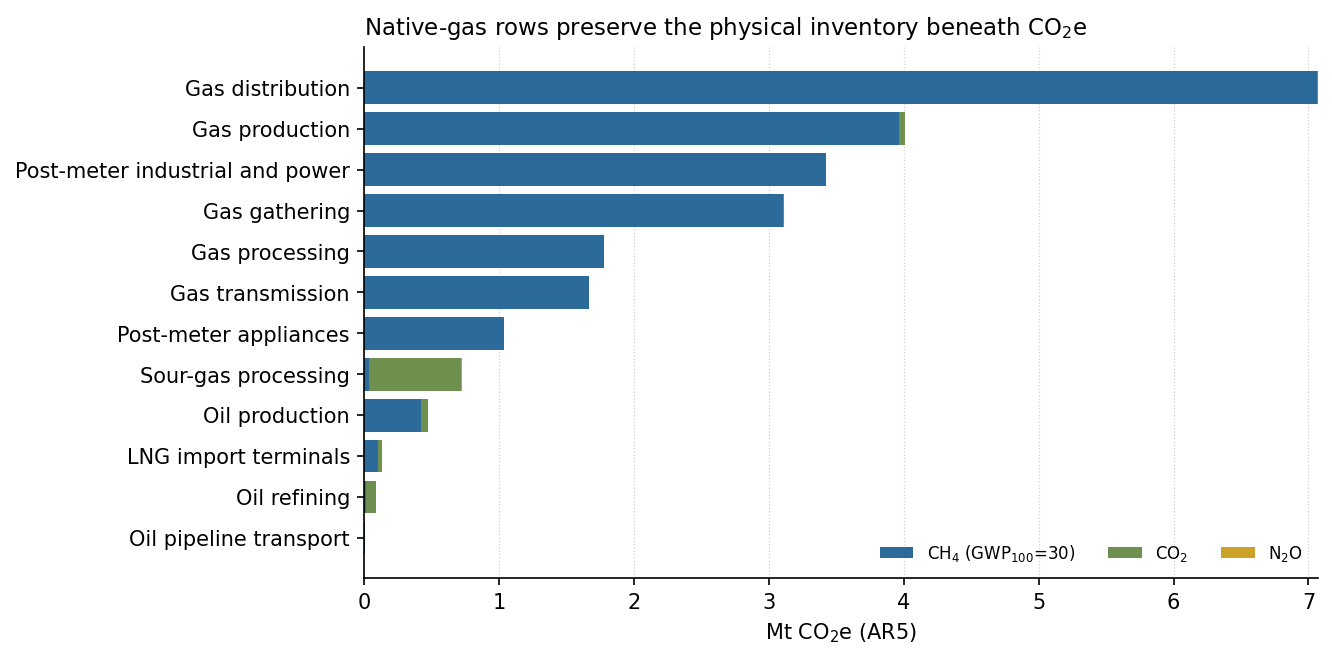
\includegraphics[width=\linewidth]{fugitives_streams.png}
\caption{Segment-level contributions by native gas.}
\label{fig:streams}
\end{figure}

The lower distribution factor reduces the national total by
\SI{5.679}{\mega\tonne}. Its selection requires more than half plastic pipe and active LDAR;
the publicly quantified \SI{8200}{\kilo\metre} of SSGCL polythene covers only
\SI{4.2}{\percent} of the national network. Halving or excluding the transferred post-meter
industrial/power factor reduces the total by \SI{1.710}{} or
\SI{3.420}{\mega\tonne}, respectively.

The named lower-practice configuration has a deterministic value of
\SI{14.894}{\mega\tonne}. A synthesized \emph{central} member---every stream with
published high/low practice bounds at their geometric mean, the retired 2006 method's
midpoint mechanism carried into the segment engine---prices \SI{17.678}{\mega\tonne},
with its own conditional interval of \SIrange{15.798}{21.309}{\mega\tonne}; it is a
named configuration, never the selection, because no measurement locates Pakistani
practice inside the bounds. The reference withholds the post-meter factor from the
fertilizer feedstock---gas chemically consumed in the reformers, not burned---and keeps the
plants' process fuel in the base. Putting the feedstock back inside the base, the membership
of earlier releases and one this paper does not defend, prices
\SI{24.694}{\mega\tonne} (the post-meter feedstock scope axis, \SI{+1.195}{\mega\tonne})
and is the top of the structural envelope; taking the
whole fertilizer class out prices \SI{23.264}{\mega\tonne} (\SI{-0.236}{\mega\tonne}).
Models retaining all public-data segments span
\SIrange{12.183}{24.694}{\mega\tonne} across the 192 segment-retaining members of the
280-configuration factorial. Permitting
proxy-supported processing and post-meter coverage to be excluded expands the envelope to
\SIrange{9.601}{24.694}{\mega\tonne}. The reference Monte Carlo has median
\SI{24.141}{\mega\tonne} and a 95\% interval of
\SIrange{21.277}{30.537}{\mega\tonne}. The national table prints the SAME
draws: the national Monte Carlo consumes this sector's persisted
\num{100000}-draw file (whose first \num{10000} draws are bit-identical to the run
above) and prints \num{24.15} for this module---the residual difference against
\num{24.141} is draw count, not convention. The 1.6-\si{\mega\tonne} family gap an
earlier edition had to explain away no longer exists;
\texttt{outputs/national\_uncertainty\_reconciliation.csv} now records the collapse. Corresponding intervals are
\SIrange{13.113}{17.311}{} for lower practices, \SIrange{18.489}{26.836}{} without industrial
post-meter emissions, and \SIrange{8.864}{10.692}{\mega\tonne} for the minimum-coverage case
(Figure~\ref{fig:uncertainty}).

\begin{figure*}[htbp]
\centering
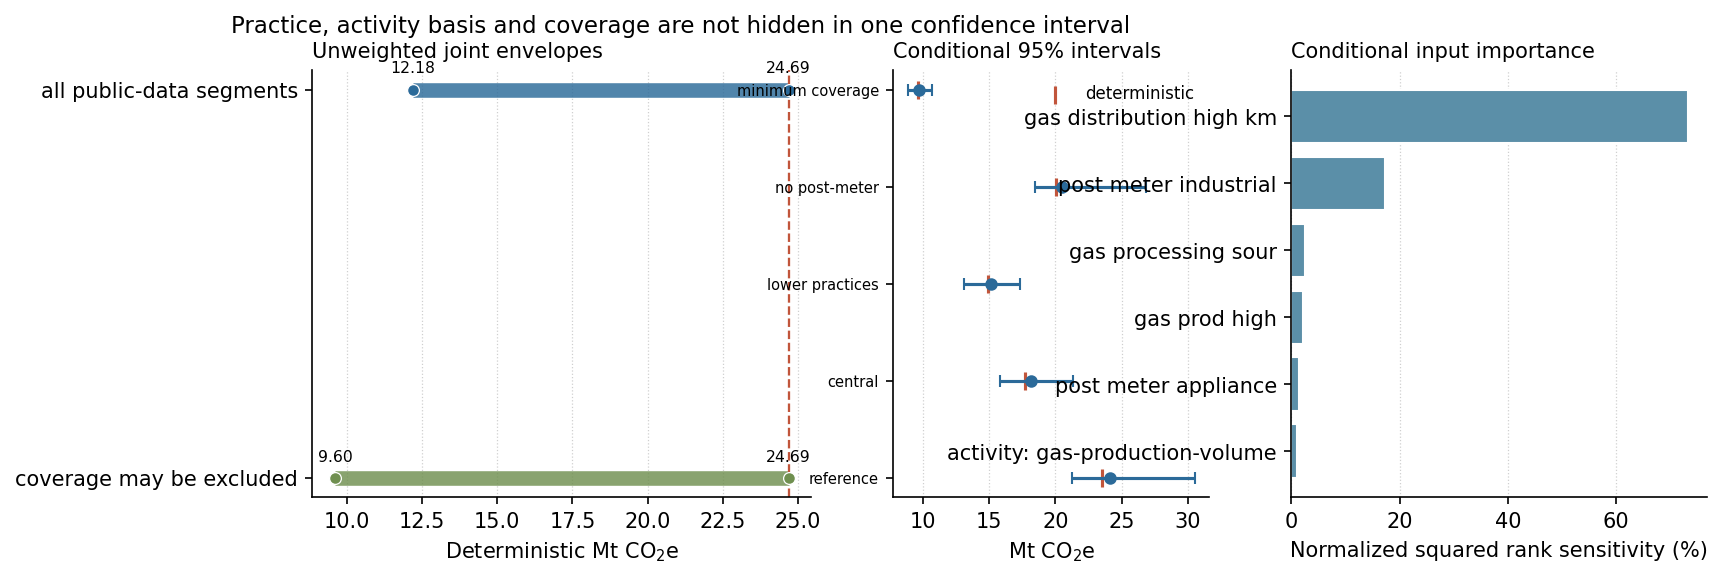
\includegraphics[width=0.96\textwidth]{fugitives_structural_uncertainty.png}
\caption{Structural envelopes, conditional parametric intervals and reference-configuration
input importance.}
\label{fig:uncertainty}
\end{figure*}

The distribution and post-meter factor groups contribute \SI{73.2}{\percent} and
\SI{17.2}{\percent} of normalized squared rank sensitivity, respectively. All remaining groups
individually contribute less than \SI{2.5}{\percent}. Alternative bounded distribution shapes
widen or shift the reference interval but leave these two measurement priorities unchanged
(Supplementary Table~S6).

\subsection{Network growth offsets declining upstream activity}

The public-data reconstruction ranges from \SI{24.384}{\mega\tonne} in FY2015--16 to a peak of
\SI{26.270}{\mega\tonne} in FY2018--19 and \SI{23.499}{\mega\tonne} in FY2023--24 (each
year's figure the reference configuration, feedstock outside the leak base in every year).
Its composition changes more clearly than its total. Upstream and processing emissions fall from
\SI{13.165}{} to \SI{10.181}{\mega\tonne} ($-22.7\%$), while network and LNG emissions rise
from \SI{6.698}{} to \SI{8.866}{\mega\tonne} ($+32.4\%$). Post-meter emissions remain nearly
constant at \SI{4.521}{} and \SI{4.453}{\mega\tonne}. Growth in pipeline length and customer
connections therefore offsets part of the decline in domestic production
(Figure~\ref{fig:official}, right).

\subsection{Physical balances and official reporting constrain magnitude}

Gross production exceeds indigenous marketable supply by \SI{11.4}{\percent}--
\SI{15.6}{\percent} across FY2021--22 to FY2023--24. The downstream balance is tighter:
indigenous marketable supply plus RLNG closes to reported supply, and the residual after
categorized consumption and UFG ranges from $-\SI{2.6}{\percent}$ to
$+\SI{1.4}{\percent}$.

Reference transmission-plus-distribution emissions are \SI{290.899}{\giga\gram} CH$_4$,
equivalent to \SI{23.8}{\percent} of reported UFG methane. Lower-practice estimates require
\SI{6.1}{\percent}; higher and lower throughput cases require \SI{18.8}{\percent} and
\SI{5.8}{\percent}. Both practice classes fit within the utility mass balance but imply sharply
different physical-loss shares (Figure~\ref{fig:ufg}).

\begin{figure*}[htbp]
\centering
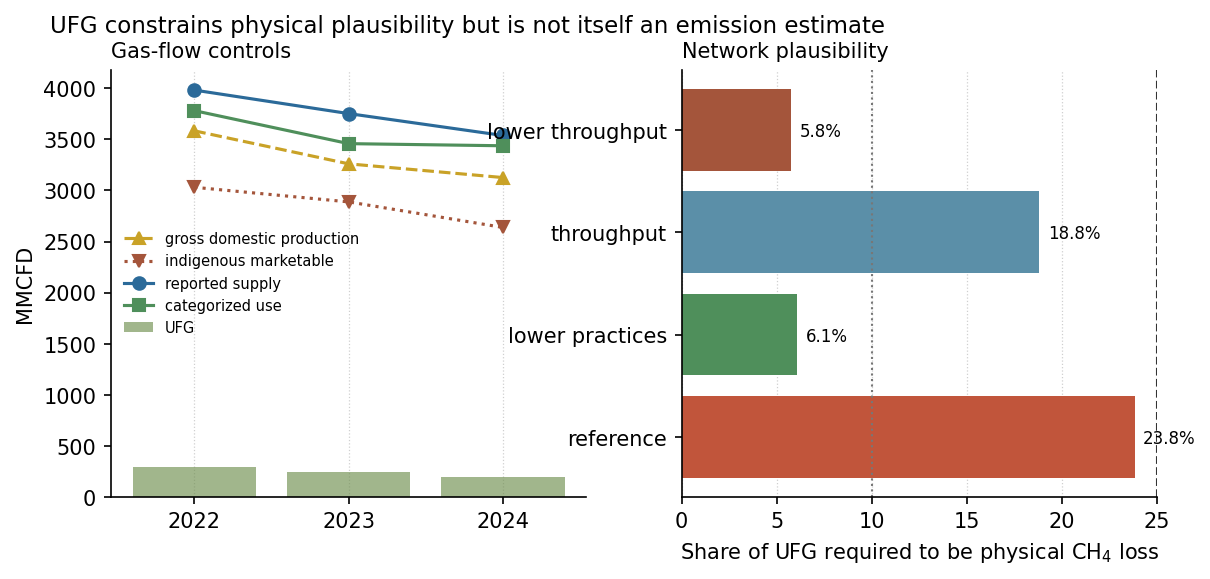
\includegraphics[width=0.94\textwidth]{fugitives_gas_flow_ufg.png}
\caption{Reported gas-flow controls (left) and the UFG share corresponding to modelled pre-meter
network methane (right).}
\label{fig:ufg}
\end{figure*}

Pakistan's 2022 CRT reports \SI{4.433}{\mega\tonne} for 1.B.2, or
\SI{4.749}{\mega\tonne} on the common GWP basis. The adjacent FY2021--22 and FY2022--23
reconstructions are \num{5.30} and \num{5.00} times this value. Fiscal-year choice changes the
reconstruction by about \SI{5.7}{\percent}.

Every CRT activity--factor row reproduces its reported native-gas result. The matched waterfall
then closes at \SI{25.187}{\mega\tonne} after harmonizing inclusive venting/flaring treatment,
replacing the oil and gas segment calculations, and adding LNG and post-meter sources. The
largest increments occur in gas production/gathering, processing, distribution and post-meter
activity (Figure~\ref{fig:official}, left).

\begin{figure*}[htbp]
\centering
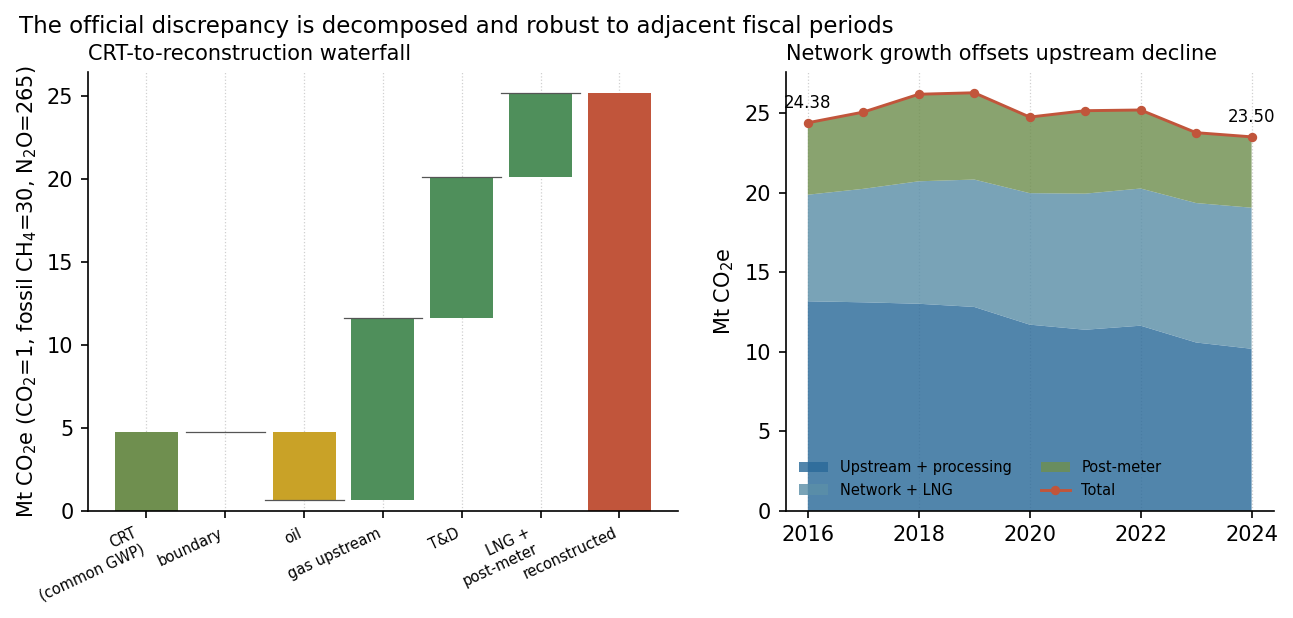
\includegraphics[width=0.95\textwidth]{fugitives_official_comparison.png}
\caption{CRT-to-reconstruction waterfall on a common GWP basis (left) and the segment-resolved
nine-year reconstruction (right).}
\label{fig:official}
\end{figure*}

\subsection{Production locates sources but weakly predicts observed intensity}

World Bank flare volume declines from \num{0.336} billion m$^3$ in 2012 to
\SI{0.130}{} in 2024. The MARS snapshot contains 20 oil-and-gas sources and 174 plumes;
19 sources occur within \SI{10}{\kilo\metre} of a World Bank flare. Matched detections occurred near
fields accounting for \SI{71.1}{\percent} of reported supply---a statement about where
the instruments matched, not about coverage: without sensor-opportunity, cloud and
detection-limit masks, a field with no matched event is unobserved, not observed-clean.

Across all 73 official fields, production has Spearman $\rho=\num{0.230}$ with VIIRS flare
volume and $\rho=\num{0.382}$ with MARS source and plume counts. Four fields overlap each
observation's production top-10. National and within-province permutations place the MARS rank
statistics at $p\leq\num{0.0013}$ and the corresponding top-field overlaps at
$p=\num{0.0065}$--$\num{0.0374}$. The VIIRS rank result is weaker, while its top-10 overlap is
less consistent with chance. Production therefore identifies broad upstream geography but
explains little of the observed intensity variation (Figure~\ref{fig:observations}).

\begin{figure*}[htbp]
\centering
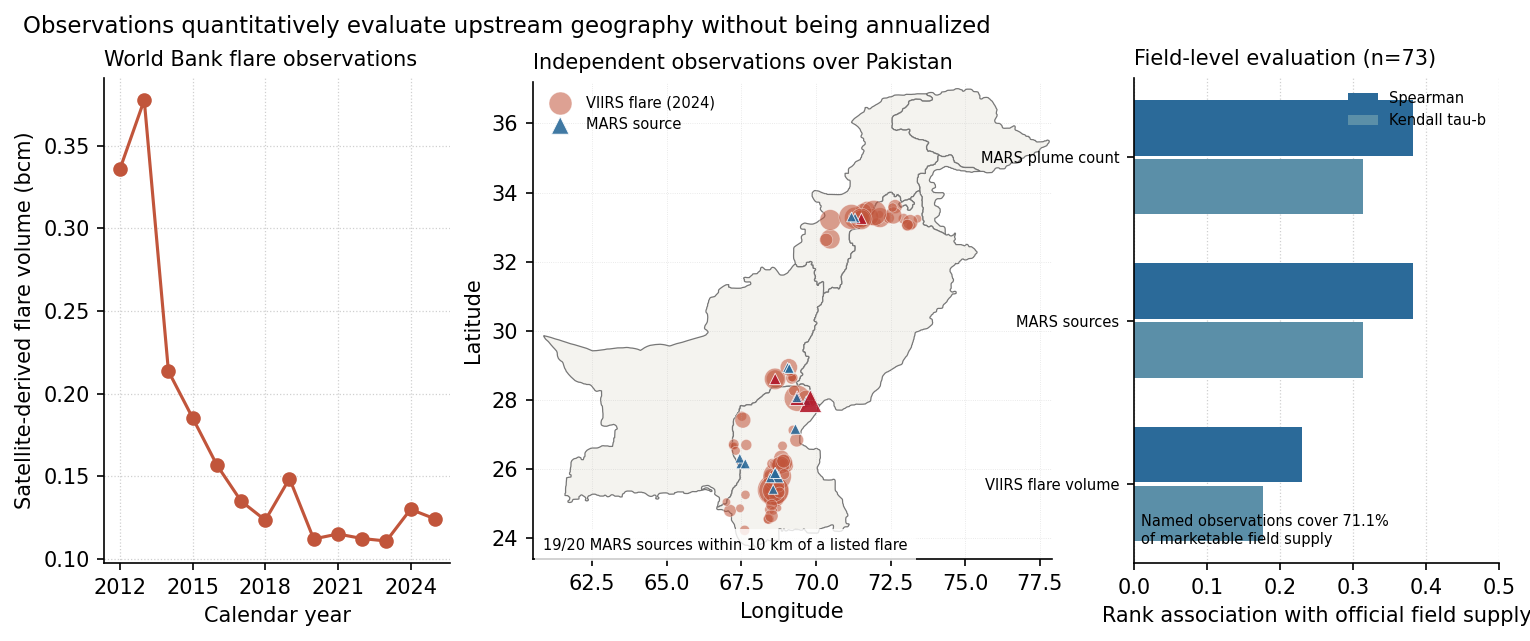
\includegraphics[width=0.95\textwidth]{fugitives_observations.png}
\caption{Annual flare volume, mapped field/flare/MARS observations and field-level ranking
diagnostics.}
\label{fig:observations}
\end{figure*}

The process-matched provincial inventory is \SI{9.99}{\mega\tonne} in Sindh,
\SI{7.77}{} in Punjab, \SI{2.86}{} in Khyber Pakhtunkhwa,
\SI{2.79}{} in Balochistan and \SI{0.09}{} in Other.
